% !TEX program = xelatex
\documentclass{beamer}
\usefonttheme[onlymath]{serif}
\setbeamerfont{footnote}{size=\tiny}

% use multiple languages
%% ---- allow CJK usage ---- %%
\usepackage[CJKspace]{xeCJK} % this should be called before Polyglossia
\setCJKmainfont{Noto Serif CJK TC}
\setCJKsansfont{Noto Sans CJK TC}
\setCJKmonofont{Noto Sans Mono CJK TC}
% \setCJKmainfont{Noto Serif JP}
% \setCJKsansfont{Noto Sans JP}
% \setCJKmonofont{Noto Sans Mono CJK JP}

%% ---- ตั้งค่าให้ตัดคำภาษาไทย ---- %%
\XeTeXlinebreaklocale "th"
\XeTeXlinebreakskip = 0pt plus 0pt % เพิ่มความกว้างเว้นวรรคให้ความยาวแต่ละบรรทัดเท่ากัน

%% ---- font settings ---- %%
\usepackage{fontspec}
\defaultfontfeatures{Mapping=tex-text} % map LaTeX formating, e.g., ``'', to match the current font
% To change the main font, uncomment one of the below command.
% \setmainfont{TeX Gyre Termes} % Free Times
% \setsansfont{TeX Gyre Heros} % Free Helvetica
% \setmonofont{TeX Gyre Cursor} % Free Courier
\newfontfamily{\thaifont}[Scale=MatchUppercase,Mapping=textext]{Laksaman} % ตั้งฟอนต์หลักภาษาไทย
\newenvironment{thailang}{\thaifont}{} % create environment for Thai language
\usepackage[Latin,Thai]{ucharclasses} % ตั้งค่าให้ใช้ "thailang" environment เฉพาะ string ที่เป็น Unicode ภาษาไทย
\setTransitionTo{Thai}{\begin{thailang}}
\setTransitionFrom{Thai}{\end{thailang}}

%% ---- spacing between lines ---- %%
\usepackage{setspace}
% \singlespacing % default setting
% \onehalfspacing % recommend using this for Thai language

%% ---- using alphabatic language ---- %%
\usepackage{polyglossia}
\setdefaultlanguage{english} % it is preferrable to set English as the main language, since the numeric system is compatible with most LaTeX features such as 'enumerate' and so on
\setotherlanguages{thai}

\AtBeginDocument\captionsthai % allow captions to be in Thai


%% ---- Title page details ---- %%
\title[]{A simple time-dependent kidney model}
\author[C. Sint]{Chanoknun Sintavanuruk 
% \\ (ชนกนันท์ สินธวานุรักษ์; 馬予棟) \inst{1} 
% \and author2 \inst{2}
}
% \institute[shortinst]{\inst{1} affiliation 
% % \and \inst{2} affiliation for author2
% }
\date{\today}

% preambles for Beamer

%% ---- math packages ---- %%
\usepackage{amsmath}
\usepackage{amssymb}
\usepackage{bm} % same functionality as \mathbf{} but for greek letters
\numberwithin{equation}{section} % equation numbers are formatted as <#Section>.<#eq in the section>
\usepackage{cancel}
\renewcommand\CancelColor{\color{red}}

%% ---- define math environment ---- %%
\usepackage{amsthm}

%% ---- hyperref settings ---- %%
% \usepackage{hyperref} % Beamer already has hyperref by default
\usepackage{url}
\usepackage{cite}
\usepackage{natbib}
\usepackage{bibentry}
\usepackage{xcolor}
\hypersetup{
    colorlinks,
    linkcolor={red!50!black},
    citecolor={blue!50!black},
    urlcolor={blue!80!black}
    }

%% ---- misc. ---- %%
\usepackage{mhchem} % use chemistry notation
\newcommand\scalemath[2]{\scalebox{#1}{\mbox{\ensuremath{\displaystyle #2}}}} % scale display math environment
\usepackage{lipsum}
\usepackage{metalogo} % for extended LaTeX logo such as XeTeX
\usepackage{subcaption} % allowing subfigure environment
% \usepackage[section]{placeins} % ensure floats do not go into the next section and allow the use of \FloatBarrier
\usepackage{graphicx} % allow cropping and rotating images

%% ---- Theme choice ---- %%
\usetheme{metropolis}
% \usetheme{Berkeley}
% \usecolortheme{beaver}
% \usecolortheme{dove}
% \usecolortheme{spruce}
% \logo{\large \XeTeX{}}

%% ---- show TOC after sections ---- %%
% \AtBeginSection[]
% {
%     \begin{frame}
%         \frametitle{Outline}
%         \tableofcontents[currentsection]
%     \end{frame}
%     }

%% ---- Show notes ---- %%
\usepackage{pgfpages}
% \setbeameroption{show notes}
% \setbeameroption{show notes on second screen=right}
% for working around text color bug when using XeLaTeX
\makeatletter 
\def\beamer@framenotesbegin{% at beginning of slide
     \usebeamercolor[fg]{normal text}
      \gdef\beamer@noteitems{}% 
      \gdef\beamer@notes{}% 
}
\makeatother

%% ---- page numbers ---- %%
% \setbeamertemplate{page number in head/foot}[totalframenumber]\setbeamertemplate{navigation symbols}{\footnotesize\usebeamertemplate{page number in head/foot}}

%% ---- figure numbering ---- %%
\setbeamertemplate{caption}[numbered]

\setbeamerfont{caption}{size=\scriptsize}

\begin{document}
% Title page frame
\begin{frame}
    \titlepage 
\end{frame}
% Remove logo from the next slides
% \logo{}

% Outline frame
\begin{frame}{Outline}
    \tableofcontents
\end{frame}

\section{Model equations}

\begin{frame}{Compartments}
    Multiphasic medulla on the domain $(0,L)$ (superficial $\to$ deep).
    \begin{enumerate}
        \item Combined interstitium-vascular compartment
        \item Descending tubule
        \item Ascending tubule
        \item Collecting tubule
    \end{enumerate}
\end{frame}

\begin{frame}{Volume density}
    \begin{equation}\label{eq:vol_conserv}
        \sum_k \alpha_k = \alpha_*
    \end{equation}
        where $\alpha_*:(0,L)\to \mathbb{R}_+$ is the total volume density.
    \pause
    \begin{align}\label{eq:volume_dynamics}
        \frac{\partial \alpha_k}{\partial t} + \frac{\partial}{\partial x}\left( \alpha_k u_k \right) &= -\gamma_kw_k,\quad k=\mathrm{D},\mathrm{A},\mathrm{C},\\
        \frac{\partial \alpha_0}{\partial t} + \frac{\partial }{\partial x}\left( \alpha_0 u_0 \right) &= \sum_{k=\mathrm{D},\mathrm{A},\mathrm{C}} \gamma_kw_k.
    \end{align}
\end{frame}

\begin{frame}{Water flow and transport}
    Poiseuille's equation:
    \begin{equation}
        \frac{\rho_k u_k}{\alpha_k} = -\frac{\partial p_k}{\partial x},\quad k=0,\mathrm{D},\mathrm{A},\mathrm{C},
    \end{equation}
    Water transport:
    \begin{equation}
        w_k := \zeta_\mathrm{w}^k\left( \psi_k - \psi_0 \right),\quad \psi_k:=p_k - \pi_k,\quad k=\mathrm{D},\mathrm{A},\mathrm{C}
    \end{equation}
    \pause
    Osmotic pressure:
    \begin{equation}
        \pi_k:= \sum_{i=\mathrm{s},\mathrm{u}}c_i^k+\frac{a_k}{\alpha_k},\quad k=0,\mathrm{D},\mathrm{A},\mathrm{C}.
    \end{equation}
\end{frame}

\begin{frame}{Pressure-compliance relationship}
    \begin{equation}
        \nu_k(p_k - p_0) = \frac{\alpha_k}{\bar{\alpha}_k} - 1,\quad k=\mathrm{D},\mathrm{A},\mathrm{C},
    \end{equation}
    $p_0$ is determined by the constaint total volume density (\ref{eq:vol_conserv}).
\end{frame}

\begin{frame}{Solute dynamics}
    Only salt and urea
    \begin{align}\label{eq:solute_dynamics}
        \frac{\partial}{\partial t}\left( \alpha_k c_i^k \right)&=-\frac{\partial}{\partial x} f_i^k - \gamma_kg_i^k,\quad k=\mathrm{D},\mathrm{A},\mathrm{C},\\
        \frac{\partial}{\partial t}\left( \alpha_0 c_i^0 \right)&=-\frac{\partial}{\partial x} f_i^0 + \sum_{k=\mathrm{D},\mathrm{A},\mathrm{C}} \gamma_k g_i^k,
    \end{align}
    \pause
    Axial solute flow:
    \begin{equation}
        f_i^k := -\alpha_kD_i^k\frac{\partial c_i^k}{\partial x}+\alpha_ku_kc_i^k,\quad k=0,\mathrm{D},\mathrm{A},\mathrm{C},
    \end{equation}
\end{frame}

\begin{frame}{solute transport}
    \begin{equation}
        g_i^k := j_i^k+h_i^k,\quad 
    \end{equation}
    \begin{equation}
        j_i^k = \zeta_i^k\left( \mu_i^k - \mu_i^0 \right),\quad ,
    \end{equation}
    \begin{equation}
        \mu_i^k:= RT\ln c_i^k,\quad 
    \end{equation}
    where $k=0,\mathrm{D},\mathrm{A},\mathrm{C}$.
\end{frame}

\begin{frame}{Boundary condition: interstitium}
    No flux at the bottom:
    \begin{align}
        u_0(t,L) &= 0,\\ 
        f_i^0(t,L)&=0,\quad i=\mathrm{s},\mathrm{u}.
    \end{align}
    Advective flow at the top:
    \begin{align}
        (\alpha_0u_0)(t,0) &= \min\left\{ 0,\frac{P_{\mathrm{v}}-p_0(t,0) }{R_{\mathrm{v}}}\right\},\\ 
        f_i^0(t,0) &= (\alpha_0 u_0 c_i^0)(t,0),\quad i=\mathrm{s},\mathrm{u}.
    \end{align}
\end{frame}

\begin{frame}{Boundary condition: input from PCT}
    \begin{align}
        (\alpha_\mathrm{D} u_\mathrm{D})(t,0) &= \mathrm{GFR}(t),\\
        f_i^\mathrm{D}(t,0) &= (\alpha_\mathrm{D}u_\mathrm{D}c_i^\mathrm{D})(t,0),\quad i=\mathrm{s,u}\\
        c_i^\mathrm{D}(t,0) &= c_{i}^{\mathrm{filtrate}}(t)
    \end{align}
\end{frame}

\begin{frame}{Boudnary condition: couplings}
    \begin{align}
        (\alpha_\mathrm{D}u_\mathrm{D}+\alpha_\mathrm{A}u_\mathrm{A})(t,L) &= 0,\\
        \quad\left( f_i^\mathrm{D}+f_i^\mathrm{A} \right)(t,L) &= 0,\\
        p_\mathrm{D}(t,L)&= p_{\mathrm{A}}(t,L),\\ 
        c_i^\mathrm{D}(t,L) &=c_i^\mathrm{A}(t,L)
    \end{align}
    and, similarly,
    \begin{align}
        (\alpha_\mathrm{A}u_\mathrm{A}+\alpha_\mathrm{C}u_\mathrm{C})(t,0) &= 0,\\
        \quad\left( f_i^\mathrm{A}+f_i^\mathrm{C} \right)(t,0) &= 0,\\
        p_\mathrm{A}(t,0)&= p_{\mathrm{C}}(t,0),\\ 
        c_i^\mathrm{A}(t,0) &=c_i^\mathrm{C}(t,0).
    \end{align}
\end{frame}

\begin{frame}{Boundary condition: papillary outflow}
    \begin{align}
        (\alpha_\mathrm{C} u_\mathrm{C} )(t,L) &= \max\left\{ 0,\frac{p_\mathrm{C} (t,L) - P_{\mathrm{p}} }{R_{\mathrm{p}}}\right\},\\
        f_i^\mathrm{C}(t,L) &= (\alpha_\mathrm{C}  u_\mathrm{C}  c_i^\mathrm{C})(t,L),\quad i=\mathrm{s},\mathrm{u}.
    \end{align}
\end{frame}

\section{Non-dimensionalization}
\begin{frame}{Rescaling}
    \begin{equation}
        x = L\hat{x},\quad t = \frac{L^2}{D_*}\hat{t},
    \end{equation}
    Unknowns:
    \begin{gather}
        \alpha_k = \bar{\alpha}\hat{\alpha},\quad c_i^k = c_*\hat{c}_i^k,\quad p_k = p_*\hat{p}_k,
        % \quad u_k = \frac{\bar{\alpha}p_*}{\rho_* L}\hat{u}
    \end{gather}    
\end{frame}

\begin{frame}{Dimensionless model}
    \begin{align}
        \frac{\partial \hat{\alpha}_k}{\partial \hat{t}}  + \mathrm{Pe}\frac{\partial}{\partial \hat{x}}\left( \hat{\alpha}_k \hat{u}_k \right) &= - \hat{w}_k,\\ \label{eq:nd_1steq}
        \frac{\partial\hat{\alpha}_0}{\partial \hat{t}}+\mathrm{Pe}\frac{\partial}{\partial \hat{x}}\left( \hat{\alpha}_0 \hat{u}_0 \right) &=\sum_k \hat{w}_k,\\
        \hat{\nu}_k\left( \hat{p}_k - \hat{p}_0 \right) &= \frac{\hat{\alpha}_k}{\hat{\bar{\alpha}}_k}-1,\\
        \hat{\alpha}_0 + \sum_{k} \hat{\alpha}_k &= \hat{\alpha}_*,\\
        \frac{\partial}{\partial \hat{t}}\left( \hat{\alpha}_k \hat{c}_i^k \right)&=-\frac{\partial}{\partial \hat{x}} \hat{f}_i^k - \hat{g}_i^k,\\
        \frac{\partial}{\partial \hat{t}}\left( \hat{\alpha}_0 \hat{c}_i^0 \right)&=-\frac{\partial}{\partial \hat{x}} \hat{f}_i^0 + \sum_k \hat{g}_i^k,
    \end{align}
\end{frame}

\begin{frame}{Dimensionless flows and transports}
    \begin{align}
        \hat{u}_\cdot &:= -\frac{\hat{\alpha}_\cdot}{\hat{\rho}_\cdot}\frac{\partial \hat{p}_\cdot}{\partial \hat{x}},\\
        \hat{f}_i^\cdot &:= -{\hat{\alpha}_\cdot}\hat{D}_\cdot \frac{\partial \hat{c}_i^\cdot}{\partial \hat{x}} + \mathrm{Pe}(\hat{\alpha}_\cdot\hat{u}_\cdot\hat{c}_i^\cdot),\\
        \hat{w}_k&:= \hat{\zeta}_\mathrm{w}^k\left( \hat{\psi}_k-\hat{\psi}_0 \right),\quad\hat{\psi}_\cdot := \hat{p}_\cdot - \hat{\pi}_.,\quad \hat{\pi}_\cdot := \frac{\hat{a}_\cdot}{\hat{\alpha}_\cdot}+\sum_i \hat{c}_i^\cdot,\\
        \hat{g}_i^k &:= \hat{j}_i^k+\hat{h}_i^k,\quad \hat{j}_i^k :=\hat{\zeta}_i^k(\hat{\mu}_i^k-\hat{\mu}_i^0),\quad \hat{\mu}_i^\cdot:=\ln \hat{c}_i^\cdot\label{eq:nd_lasteq}
    \end{align}
        for $k=\mathrm{D},\mathrm{A},\mathrm{C}$ and $i=\mathrm{s},\mathrm{u}$.
\end{frame}

\begin{frame}{Parameters}
    \begin{gather}
        \mathrm{Pe} = \frac{\bar{\alpha}p_*/\rho_*}{D_*},\quad \hat{\rho}_\cdot = \frac{\rho_\cdot}{\rho_*},\quad \hat{\nu}_k = p_*\nu_k,\quad \hat{\bar{\alpha}}_\cdot = \frac{\bar{\alpha}_\cdot}{\bar{\alpha}},\quad \hat{\alpha}_* = \frac{\alpha_*}{\bar{\alpha}}\\
        \hat{a}_\cdot = \frac{a_\cdot}{\bar{\alpha}c_*},\quad
        \hat{D}_\cdot = \frac{D_\cdot}{D_*},\quad \hat{\zeta}_\mathrm{w}^k = \frac{\gamma_k c_*L^2}{\bar{\alpha}D_*}\zeta_\mathrm{w}^k,\quad\hat{\zeta}_i^k = \frac{\gamma_kRT L^2}{\bar{\alpha}c_* D_*}\zeta_i^k,
    \end{gather}
\end{frame}

\section{Simulation}

\begin{frame}{Specification}
    \begin{itemize}
        \item $\alpha_* \equiv 1$, $\bar{\alpha}_k = 1/4$, and $\nu_k = 0.01$ for $k=\mathrm{D},\mathrm{A},\mathrm{C}$.
        \item Suppose that $D_\mathrm{s}^k = D_{\mathrm{u}}^k = 1$, $\mathrm{Pe} = 20$, $\rho_k = 1$ for all $k$
        \item Only immobile solute in the interstitium, i.e., $a_0 = 1/2$ and $a_k = 0$.
        \item $R_\mathrm{v} = R_\mathrm{p} = 1$ and $P_\mathrm{v} = P_\mathrm{p} = 1$
    \end{itemize}
\end{frame}

\begin{frame}{Solute transports}
    Passive transport of salt only in the descending and the ascending tubules: $\zeta_{\mathrm{s}}^\mathrm{D} = \zeta_{\mathrm{s}}^\mathrm{A} = 1$ and $\zeta_{\mathrm{s}}^\mathrm{C} = 0$.

    \pause
    Active transport:
    \begin{equation}
        h_\mathrm{s}^\mathrm{A} = \begin{cases}
            h_*c_\mathrm{s}^\mathrm{A},\quad  &\text{in}\quad (0,\frac{1}{2}),\\
            0\quad &\text{in}\quad [\frac{1}{2},1),
        \end{cases}
    \end{equation}

    \pause
    Urea permeable in the inner medulla: $\zeta_{\mathrm{u}}^k = 10$ for all $k$ and $x\in (\frac{1}{2},1)$ and $\zeta_{\mathrm{u}}^k =0$ elsewhere.

    \pause
    High water permeability in the descending tubule, $\zeta_\mathrm{w}^\mathrm{D} = 100$, while the ascending tubule is completely insulated: $\zeta_\mathrm{w}^\mathrm{A} = 0$.
\end{frame}

\begin{frame}{ADH on/off}
    \begin{itemize}
        \item ADH on: $\zeta_{\mathrm{w}}^\mathrm{C} = 0$
        \item ADH off: $\zeta_{\mathrm{w}}^\mathrm{C} = 50$
    \end{itemize}
\end{frame}

\begin{frame}{ADH off}
    
\begin{columns}[T]

    \begin{column}{0.5\textwidth}
    \begin{figure}
        \centering
        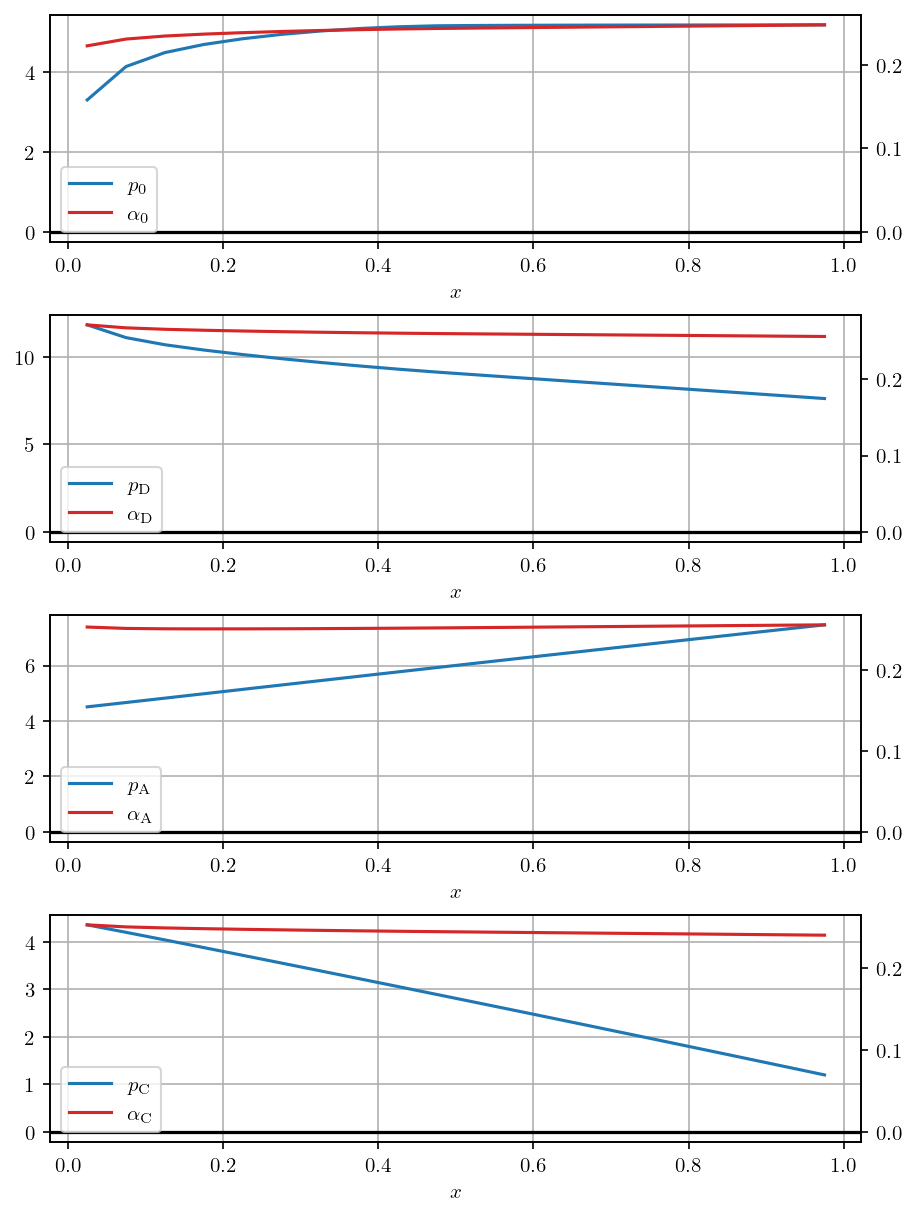
\includegraphics[width=\textwidth]{results/4-7-2023/noADH_p_alpha.png}
    \end{figure}
    \end{column}
    
    \begin{column}{0.5\textwidth}
        \begin{figure}
            \centering
            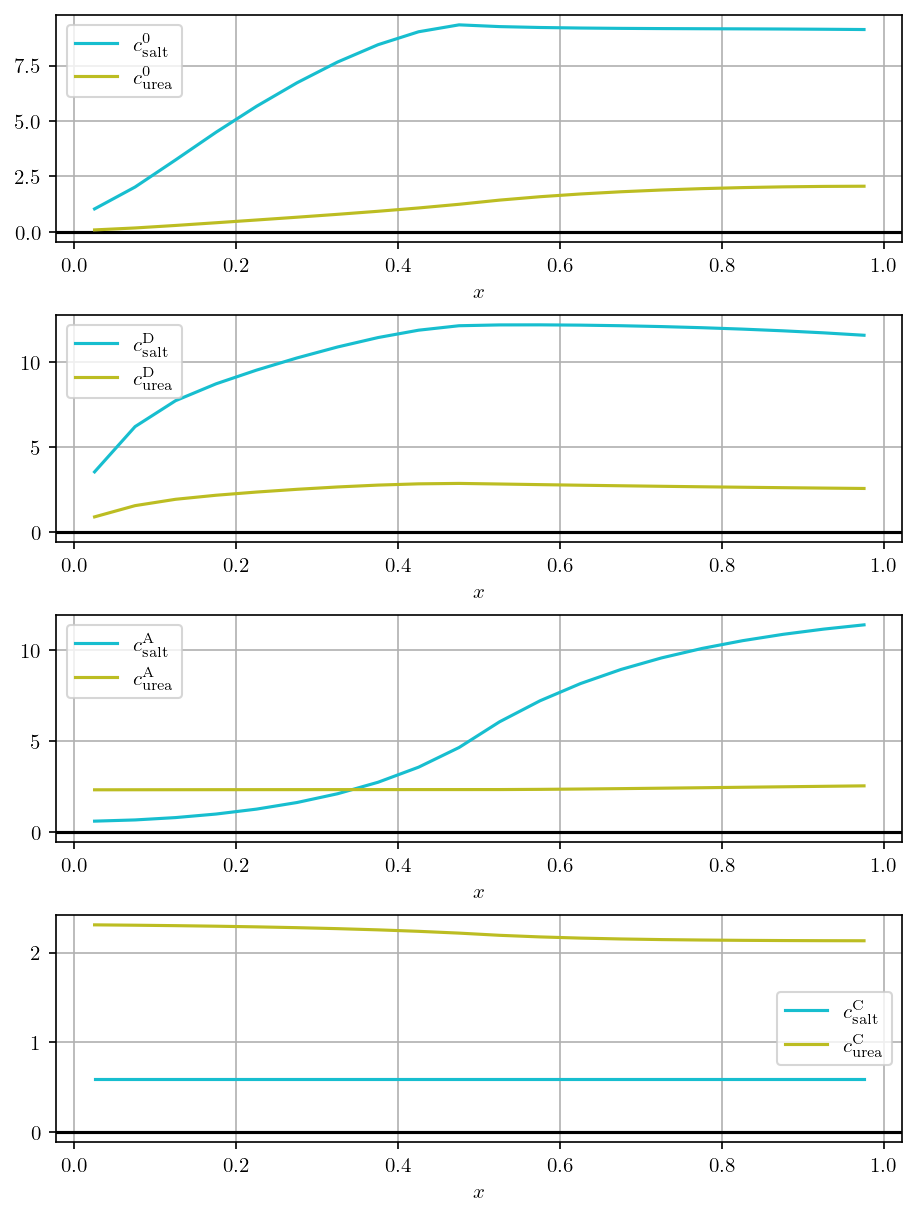
\includegraphics[width=\textwidth]{results/4-7-2023/noADH_c.png}
        \end{figure}
    \end{column}

\end{columns}
    
\end{frame}
\begin{frame}{ADH on}
    
\begin{columns}[T]

    \begin{column}{0.5\textwidth}
    \begin{figure}
        \centering
        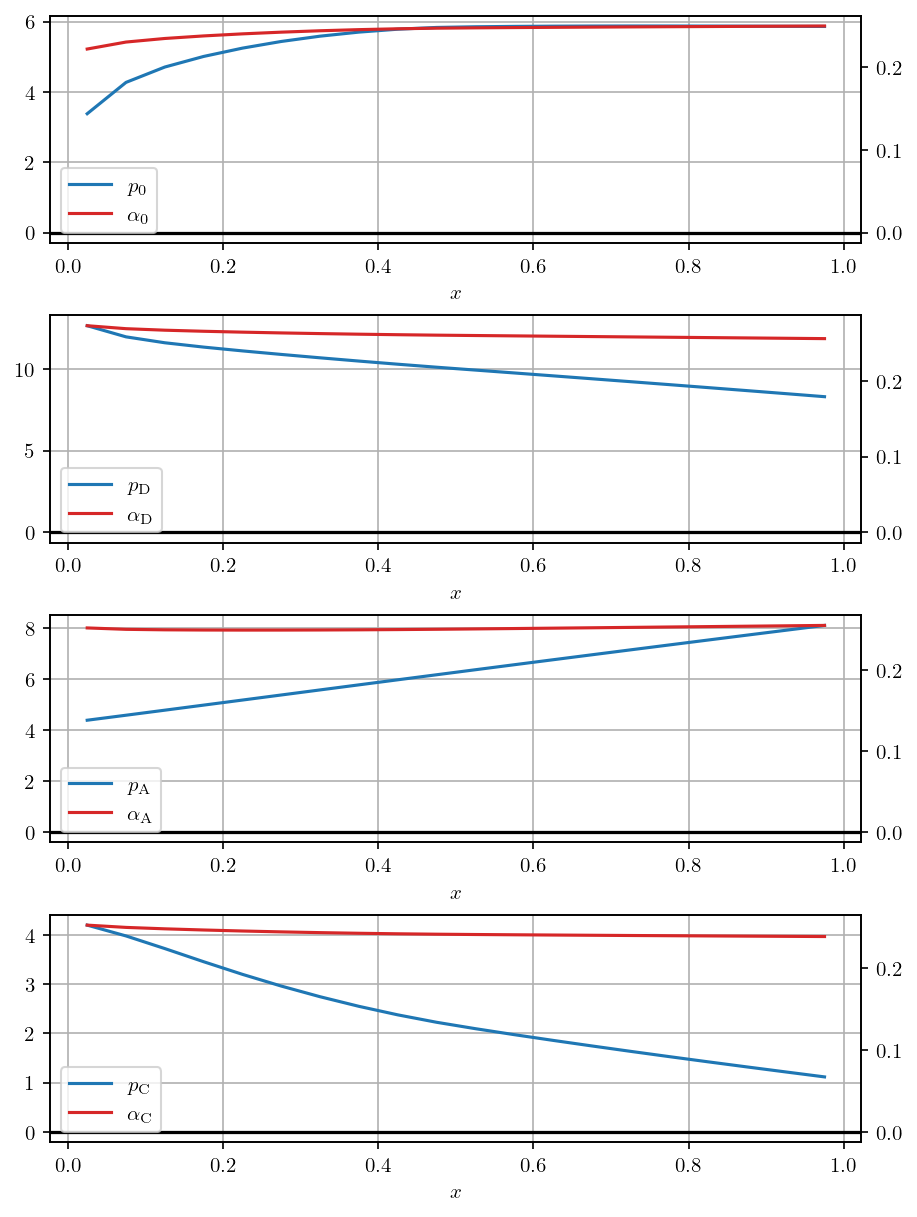
\includegraphics[width=\textwidth]{results/4-7-2023/ADH_p_alpha.png}
    \end{figure}
    \end{column}
    
    \begin{column}{0.5\textwidth}
        \begin{figure}
            \centering
            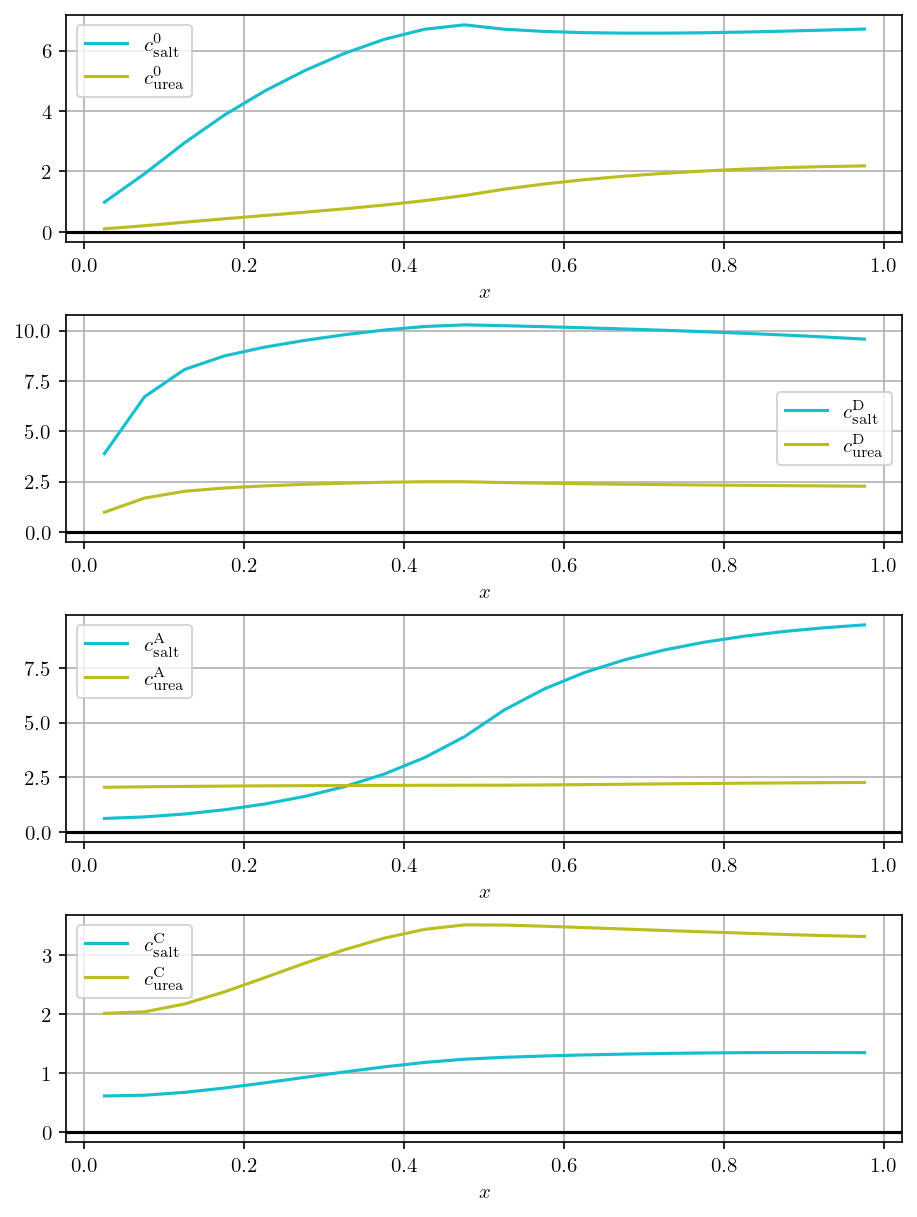
\includegraphics[width=\textwidth]{results/4-7-2023/ADH_c.png}
        \end{figure}
    \end{column}

\end{columns}
    
\end{frame}

\begin{frame}[allowframebreaks]{References}
    \bibliographystyle{plainnat}
    \tiny\bibliography{bibliography}
\end{frame}

\end{document}